\documentclass[11pt]{article}

\usepackage[margin=1in]{geometry}
\usepackage{amsmath,amssymb,mathtools,bm}
\usepackage{booktabs,array,longtable}
\usepackage{xcolor}
\usepackage{hyperref}
\usepackage{listings}
\usepackage{tikz}
\usetikzlibrary{arrows.meta,positioning,fit}

\definecolor{codeblue}{RGB}{32,74,135}
\definecolor{codegreen}{RGB}{38,122,72}
\definecolor{codegray}{RGB}{95,99,104}
\definecolor{back}{RGB}{247,248,250}
\hypersetup{colorlinks=true,linkcolor=codeblue,urlcolor=codeblue,citecolor=codegreen}
\lstset{
  language=Python,
  basicstyle=\ttfamily\small,
  keywordstyle=\color{codeblue}\bfseries,
  commentstyle=\color{codegreen},
  stringstyle=\color{purple},
  backgroundcolor=\color{back},
  frame=single,
  breaklines=true,
  showstringspaces=false,
  columns=fullflexible
}

\newcommand{\R}{\mathbb{R}}
\newcommand{\softmax}{\operatorname{softmax}}
\newcommand{\diag}{\operatorname{diag}}
\newcommand{\grad}{\nabla}

\title{Attention Is All You Need\\
\large Mathematical Intuition, a NumPy Implementation, and Manual Backpropagation}
\author{Study notes for the Consciousness Project}
\date{\today}

\begin{document}
\maketitle
\tableofcontents
\newpage

\section{Purpose and learning goals}

These notes connect the Transformer paper \emph{Attention Is All You Need} \cite{vaswani2017attention}
to a small causal language model implemented from first principles. The goal is not merely to call a
library function. It is to understand what every matrix represents, why its dimensions match, how the
loss assigns credit to parameters, and why repeated gradient updates constitute learning.

After reviewing this document, one should be able to:
\begin{enumerate}
  \item explain tokens, embeddings, queries, keys, values, logits, and causal masking;
  \item derive scaled dot-product attention and row-wise softmax;
  \item construct the complete forward pass from text to next-token loss;
  \item derive the backward pass through the vocabulary projection and attention;
  \item explain gradient descent, mini-batch training, and the computational cost of attention;
  \item identify what the toy experiment proves, what it does not prove, and how to improve it.
\end{enumerate}

\section{What problem did the paper address?}

Earlier sequence-to-sequence systems usually relied on recurrent or convolutional networks. Recurrent
models process positions sequentially, which limits parallel computation and makes long dependency paths.
The Transformer removes recurrence and uses attention to connect positions directly. The paper's central
claim is that an architecture based primarily on attention can train more efficiently while obtaining
strong translation quality.

Three distinct claims should not be conflated:
\begin{itemize}
  \item \textbf{Parallelism:} all token representations in a layer can be computed simultaneously during training.
  \item \textbf{Path length:} any two positions can interact through one self-attention operation.
  \item \textbf{Quality:} the reported translation systems achieved strong BLEU scores at favorable training cost.
\end{itemize}

BLEU is an automatic translation metric based on modified $n$-gram precision and a brevity penalty. It is
not ``percent human quality.'' FLOPs are floating-point operations and provide an approximate measure of
computational work. Neither metric alone gives a complete account of language quality or efficiency.

\section{From text to vectors}

\subsection{Tokens and token IDs}

A tokenizer splits text into units called \emph{tokens}. Modern tokenizers usually operate on subwords or
byte-based pieces rather than assigning one ID to every English word. A vocabulary maps each token to an
integer ID. For the toy sentence
\[
  \texttt{I love love math .}
\]
we used
\[
\{\texttt{I}:0,\;\texttt{love}:1,\;\texttt{math}:2,\;\texttt{.}:3\},
\qquad [0,1,1,2,3].
\]
An ID is an address, not a meaningful numerical magnitude: token 3 is not ``three times'' token 1.

\subsection{Embedding lookup}

Let $E\in\R^{V\times d_{\rm model}}$ be an embedding table. Row $E_t$ is the learned vector associated
with token ID $t$. If the ID sequence is $(t_1,\ldots,t_n)$, then
\[
  X_i=E_{t_i},\qquad X\in\R^{n\times d_{\rm model}}.
\]
Repeated tokens initially retrieve the same row. Context later makes their hidden representations differ.
The entries of $E$ are initialized and then learned by gradient descent; they are not supplied by a dictionary.

\subsection{Position information}

Attention alone is permutation-equivariant, so the original Transformer adds sinusoidal positional encodings:
\begin{align}
  \mathrm{PE}(pos,2i)&=\sin\!\left(pos/10000^{2i/d_{\rm model}}\right),\\
  \mathrm{PE}(pos,2i+1)&=\cos\!\left(pos/10000^{2i/d_{\rm model}}\right).
\end{align}
Thus the layer input is token embedding plus position encoding. Our toy calculation omitted positional
encoding, which is one reason it is an educational model rather than a complete Transformer.

\section{Queries, keys, and values}

From the same input $X$, learned projections create
\[
  Q=XW_Q,\qquad K=XW_K,\qquad V=XW_V.
\]
The interpretations are:
\begin{itemize}
  \item a \textbf{query} describes what the destination position is looking for;
  \item a \textbf{key} describes what a source position offers for comparison;
  \item a \textbf{value} contains the information contributed if that source is selected.
\end{itemize}
These roles are learned. We do not manually label a dimension as ``subject'' or ``verb.'' Training discovers
features that help predict the targets.

\section{Scaled dot-product attention}

For one head,
\begin{equation}
  S=\frac{QK^\top}{\sqrt{d_k}}+M,\qquad
  A=\softmax_{\rm row}(S),\qquad
  O=AV.
  \label{eq:attention}
\end{equation}
The entry
\[
  S_{ij}=\frac{q_i^\top k_j}{\sqrt{d_k}}+M_{ij}
\]
measures how compatible destination $i$ is with source $j$. Row $i$ considers all sources for one query.

If query and key components are roughly independent with unit variance, the unscaled dot product has
variance proportional to $d_k$. Large magnitudes can saturate softmax and produce very small gradients.
Dividing by $\sqrt{d_k}$ keeps the scale more stable.

\subsection{Causal masking}

For autoregressive prediction,
\[
  M_{ij}=\begin{cases}
  0,&j\leq i,\\
  -\infty,&j>i.
  \end{cases}
\]
Since $e^{-\infty}=0$, future positions receive zero probability. The mask prevents information leakage:
when predicting the next token, the model may use only the prefix already available.

\subsection{Softmax as a Gibbs distribution}

For a score row $s$ and temperature $\tau>0$,
\[
  p_j=\frac{e^{s_j/\tau}}{\sum_k e^{s_k/\tau}}.
\]
As $\tau\to0^+$, probability concentrates on the maximum score. As $\tau\to\infty$, the distribution
approaches uniform. Numerically stable softmax subtracts the maximum score:
\[
  \softmax(s)_j=\frac{e^{s_j-m}}{\sum_k e^{s_k-m}},\qquad m=\max_k s_k.
\]
The subtraction changes neither probability because the common factor $e^{-m}$ cancels.

\section{Multi-head attention and the Transformer block}

One head may learn one family of relationships. Multi-head attention uses separate projections:
\begin{align}
  \mathrm{head}_h&=\mathrm{Attention}(XW_Q^{(h)},XW_K^{(h)},XW_V^{(h)}),\\
  \mathrm{MHA}(X)&=\mathrm{Concat}(\mathrm{head}_1,\ldots,\mathrm{head}_H)W_O.
\end{align}
The original encoder layer combines multi-head self-attention and a position-wise feed-forward network,
with residual connections and layer normalization. Its feed-forward sublayer is
\[
  \mathrm{FFN}(x)=\max(0,xW_1+b_1)W_2+b_2.
\]
The decoder adds causal masking and, in the original encoder--decoder translation architecture, cross-attention
from decoder queries to encoder keys and values.

\begin{figure}[ht]
\centering
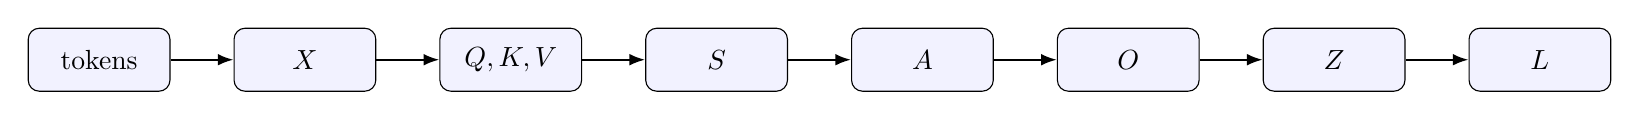
\begin{tikzpicture}[node distance=7mm and 8mm,box/.style={draw,rounded corners,fill=blue!5,minimum width=18mm,minimum height=8mm},arr/.style={-{Latex[length=2mm]},thick}]
  \node[box] (tok) {tokens};
  \node[box,right=of tok] (x) {$X$};
  \node[box,right=of x] (qkv) {$Q,K,V$};
  \node[box,right=of qkv] (s) {$S$};
  \node[box,right=of s] (a) {$A$};
  \node[box,right=of a] (o) {$O$};
  \node[box,right=of o] (z) {$Z$};
  \node[box,right=of z] (l) {$L$};
  \draw[arr] (tok)--(x); \draw[arr] (x)--(qkv); \draw[arr] (qkv)--(s);
  \draw[arr] (s)--(a); \draw[arr] (a)--(o); \draw[arr] (o)--(z); \draw[arr] (z)--(l);
\end{tikzpicture}
\caption{The toy model's forward computational graph. Backpropagation traverses it from right to left.}
\end{figure}

\section{From attention output to next-token probabilities}

The vocabulary projection produces logits
\[
  Z=OW_{\rm vocab},\qquad Z\in\R^{n\times V}.
\]
A logit is an unnormalized score. It is not itself a probability. Row-wise softmax gives
\[
  P_{ij}=\frac{e^{Z_{ij}}}{\sum_{k=1}^{V}e^{Z_{ik}}}.
\]
Row $i$ is the predicted distribution for the token following prefix position $i$. If the correct target ID
at row $i$ is $t_i$, only $P_{i,t_i}$ is the probability assigned to the observed answer.

The mean negative log-likelihood is
\begin{equation}
  L=-\frac1N\sum_{i=1}^N\log P_{i,t_i}.
  \label{eq:loss}
\end{equation}
The logarithm converts products of probabilities into sums, heavily penalizes confident wrong predictions,
and corresponds to maximum likelihood estimation. Calling this merely ``information lost'' is incomplete:
cross-entropy measures how surprising the observed targets are under the model.

\section{Gradient descent and backpropagation}

\subsection{Their different jobs}

Backpropagation computes derivatives by applying the chain rule backward through the computational graph:
\[
  \text{backpropagation: calculate }\grad_\theta L.
\]
Gradient descent uses those derivatives to change parameters:
\[
  \text{gradient descent: }\theta\leftarrow\theta-\eta\grad_\theta L.
\]
The gradient points in the direction of steepest local increase, so its negative is a local downhill direction.
The learning rate $\eta$ controls step size. Every update invalidates the old gradient, so a new forward and
backward pass is required.

\subsection{Softmax--cross-entropy derivative}

For one row with one-hot target $y$,
\[
  L=-\sum_jy_j\log p_j=-z_t+\log\sum_ke^{z_k}.
\]
Therefore
\[
  \frac{\partial L}{\partial z_j}=p_j-y_j.
\]
For a mean over $N$ training positions,
\begin{equation}
  G\equiv\frac{\partial L}{\partial Z}=\frac{P-Y}{N}.
  \label{eq:G}
\end{equation}
Every row of $G$ sums to zero because both $P_i$ and $Y_i$ sum to one. Equivalently, softmax is unchanged
when the same constant is added to all logits.

\section{Complete manual backward pass}

We use the convention that a gradient has the same shape as its variable. Let $N$ be the number of supervised
query rows and let the subscript ``train'' select those rows.

\subsection{Vocabulary projection}

From $Z=O_{\rm train}W_{\rm vocab}$ and Eq.~\eqref{eq:G},
\begin{align}
  \grad_{W_{\rm vocab}}L&=O_{\rm train}^\top G,\\
  \grad_{O_{\rm train}}L&=GW_{\rm vocab}^\top.
\end{align}

\subsection{Weighted values}

From $O_{\rm train}=A_{\rm train}V$,
\begin{align}
  \grad_A L&=(\grad_O L)V^\top,\\
  \grad_V L&=A_{\rm train}^\top(\grad_O L).
\end{align}

\subsection{Attention softmax}

For one row $a=\softmax(s)$,
\[
  \frac{\partial a_j}{\partial s_k}=a_j(\delta_{jk}-a_k).
\]
The diagonal case is $a_j(1-a_j)$; the off-diagonal case is $-a_ja_k$ because increasing one score
reduces the other normalized probabilities. If $g^A=\partial L/\partial a$, then
\begin{equation}
  g^S_k=a_k\left(g^A_k-\sum_j a_jg^A_j\right).
  \label{eq:softmaxback}
\end{equation}
In matrix notation this is an elementwise operation applied independently to each row. The rows of $\grad_S L$
sum to zero. Masked probabilities are zero, so no gradient passes through forbidden attention connections.

\subsection{Score product}

From $S_{\rm train}=Q_{\rm train}K^\top/\sqrt{d_k}+M$,
\begin{align}
  \grad_Q L&=\frac{(\grad_S L)K}{\sqrt{d_k}},\\
  \grad_K L&=\frac{(\grad_S L)^\top Q_{\rm train}}{\sqrt{d_k}}.
\end{align}
The mask is constant and has no trainable gradient.

\subsection{Projection matrices and input representation}

Because $Q=XW_Q$, $K=XW_K$, and $V=XW_V$,
\begin{align}
  \grad_{W_Q}L&=X_{\rm train}^\top\grad_Q L,\\
  \grad_{W_K}L&=X^\top\grad_K L,\\
  \grad_{W_V}L&=X^\top\grad_V L.
\end{align}
The input receives three gradient paths, which must be added:
\begin{equation}
  \grad_XL=(\grad_Q L)W_Q^\top+(\grad_K L)W_K^\top+(\grad_V L)W_V^\top,
\end{equation}
with the query contribution placed only in supervised query rows.

For the lookup $X_i=E_{t_i}$, each $\grad_{X_i}L$ is accumulated into row $t_i$ of $\grad_E L$.
If a token occurs twice, both occurrences contribute to the same embedding row. Assignment would incorrectly
overwrite one occurrence; accumulation is essential.

\section{Complete NumPy reference implementation}

The following compact program implements the mathematical chain above. It intentionally exposes intermediate
variables for study; production code would use automatic differentiation.

\begin{lstlisting}
import numpy as np

def softmax_rows(scores):
    row_max = np.max(scores, axis=1, keepdims=True)
    exp_scores = np.exp(scores - row_max)
    return exp_scores / np.sum(exp_scores, axis=1, keepdims=True)

def attention(X, W_Q, W_K, W_V):
    Q = X @ W_Q
    K = X @ W_K
    V = X @ W_V
    dk = Q.shape[1]
    n = X.shape[0]

    raw_scores = (Q @ K.T) / np.sqrt(dk)
    mask = np.triu(np.full((n, n), -np.inf), k=1)
    A = softmax_rows(raw_scores + mask)
    O = A @ V
    return Q, K, V, raw_scores, A, O

def loss_and_gradients(token_ids, target_ids, E, W_Q, W_K,
                       W_V, W_vocab):
    N = len(target_ids)
    X = E[token_ids]
    Q, K, V, S, A, O = attention(X, W_Q, W_K, W_V)

    # Forward pass from attention outputs to mean next-token loss.
    O_train = O[:N]
    A_train = A[:N]
    Q_train = Q[:N]
    X_train = X[:N]
    Z = O_train @ W_vocab
    P = softmax_rows(Z)

    Y = np.zeros_like(P)
    for i, target in enumerate(target_ids):
        Y[i, target] = 1.0

    correct_p = P[np.arange(N), target_ids]
    loss = np.mean(-np.log(correct_p))

    # Backward pass.
    G = (P - Y) / N                         # dL/dZ
    gW_vocab = O_train.T @ G                # dL/dW_vocab
    gO = G @ W_vocab.T                      # dL/dO
    gA = gO @ V.T                           # dL/dA
    gV = A_train.T @ gO                     # dL/dV

    row_dot = np.sum(gA * A_train, axis=1, keepdims=True)
    gS = A_train * (gA - row_dot)            # dL/dS

    dk = Q.shape[1]
    gQ = (gS @ K) / np.sqrt(dk)
    gK = (gS.T @ Q_train) / np.sqrt(dk)

    gW_Q = X_train.T @ gQ
    gW_K = X.T @ gK
    gW_V = X.T @ gV

    gX_Q = np.zeros_like(X, dtype=float)
    gX_Q[:N] = gQ @ W_Q.T
    gX = gX_Q + gK @ W_K.T + gV @ W_V.T

    gE = np.zeros_like(E, dtype=float)
    for position, token_id in enumerate(token_ids):
        gE[token_id] += gX[position]

    grads = {
        "E": gE, "W_Q": gW_Q, "W_K": gW_K,
        "W_V": gW_V, "W_vocab": gW_vocab
    }
    return loss, P, A, grads

# Each parameter must be floating point before small updates are applied.
params = {
    "E": E.astype(float).copy(),
    "W_Q": W_Q.astype(float).copy(),
    "W_K": W_K.astype(float).copy(),
    "W_V": W_V.astype(float).copy(),
    "W_vocab": W_vocab.astype(float).copy(),
}

learning_rate = 0.1
loss_history = []

for step in range(1000):
    loss, P, A, grads = loss_and_gradients(
        token_ids, target_ids,
        params["E"], params["W_Q"], params["W_K"],
        params["W_V"], params["W_vocab"]
    )
    loss_history.append(loss)

    for name in params:
        params[name] -= learning_rate * grads[name]

    if loss < 1e-3:
        break

print("steps:", step + 1)
print("final loss:", loss)
\end{lstlisting}

\section{What our numerical experiment established}

Using hand-selected toy matrices, the initial mean loss was approximately
\[
  1.76959.
\]
Updating only $W_{\rm vocab}$ once reduced it to approximately $1.61121$. Repeated updates of that matrix
could drive the training loss near $0.006$, demonstrating optimization but largely memorizing one sequence.
After deriving every gradient, one simultaneous update of all parameter matrices reduced the loss to
\[
  1.66621.
\]
This decrease is a useful consistency check for the entire backward pass.

\subsection{Training the complete toy model}

We then placed the entire forward pass, backward pass, and simultaneous parameter update inside a
1,000-step full-batch gradient-descent loop. All five parameter arrays---$E$, $W_Q$, $W_K$, $W_V$, and
$W_{\rm vocab}$---were updated with learning rate $\eta=0.1$. The measured losses were:

\begin{center}
\begin{tabular}{rr@{\qquad}rr}
\toprule
Step & Loss & Step & Loss\\
\midrule
0   & 1.769590 & 500 & 0.013696\\
100 & 0.513505 & 600 & 0.008181\\
200 & 0.200898 & 700 & 0.005599\\
300 & 0.100495 & 800 & 0.004159\\
400 & 0.029505 & 900 & 0.003261\\
\bottomrule
\end{tabular}
\end{center}

The final recorded loss at step 999 was $0.002661$. Thus the complete manually differentiated model,
rather than only its vocabulary projection, learned to assign nearly all probability to the four training
targets.

\begin{figure}[ht]
\centering
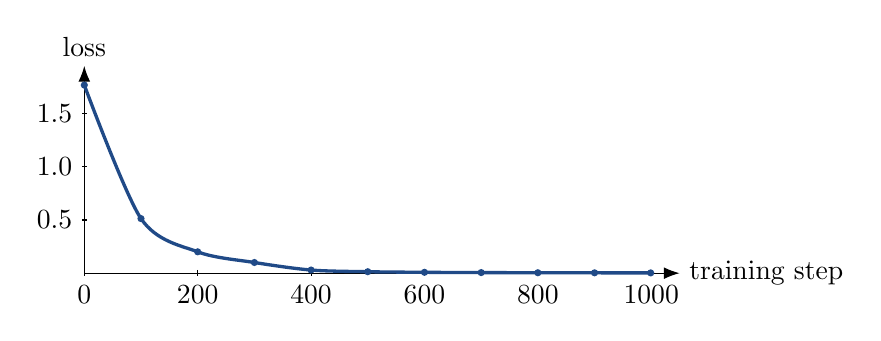
\begin{tikzpicture}[x=0.72cm,y=1.35cm]
  \draw[-{Latex[length=2mm]}] (0,0) -- (10.5,0) node[right] {training step};
  \draw[-{Latex[length=2mm]}] (0,0) -- (0,1.95) node[above] {loss};
  \foreach \x/\lab in {0/0,2/200,4/400,6/600,8/800,10/1000}
    \draw (\x,0.03)--(\x,-0.03) node[below] {\lab};
  \foreach \y/\lab in {0.5/0.5,1/1.0,1.5/1.5}
    \draw (0.04,\y)--(-0.04,\y) node[left] {\lab};
  \draw[codeblue,very thick]
    plot[smooth] coordinates {
      (0,1.769590) (1,0.513505) (2,0.200898) (3,0.100495)
      (4,0.029505) (5,0.013696) (6,0.008181) (7,0.005599)
      (8,0.004159) (9,0.003261) (9.99,0.002661)
    };
  \foreach \x/\y in {
    0/1.769590,1/0.513505,2/0.200898,3/0.100495,4/0.029505,
    5/0.013696,6/0.008181,7/0.005599,8/0.004159,9/0.003261,9.99/0.002661}
    \fill[codeblue] (\x,\y) circle (1.3pt);
\end{tikzpicture}
\caption{Measured 100-step checkpoints of mean next-token cross-entropy while all toy-model parameters are trained. The repository also contains the full-resolution exported curve.}
\label{fig:learningcurve}
\end{figure}

The full-resolution history contained 104 individual steps at which the loss increased, even though every
100-step checkpoint decreased. This is compatible with gradient descent: $-\grad L$ is a downhill direction
for an infinitesimal displacement, while the finite update $-\eta\grad L$ can overshoot a locally favorable
distance. The model is also nonconvex and all parameter matrices change together. Reducing $\eta$ usually
makes the trajectory smoother at the cost of slower progress. These temporary increases should not be
confused with predictive entropy; the plotted quantity is cross-entropy against the observed targets.

The toy keys happened to be identical. Because each row of $\grad_S L$ sums to zero,
\[
  \grad_Q L=\frac{\grad_S L\,K}{\sqrt{d_k}}\approx0
\]
in this special symmetric example. This is not a general property of attention. The final token's embedding
gradient was zero because it was not a supervised query and causal masking prevented earlier queries from
using it as a key or value.

\section{Why large-scale training is expensive}

For sequence length $n$, the score matrix has $n^2$ entries. Standard attention therefore costs roughly
$O(n^2d_k)$ operations and $O(n^2)$ attention memory per head. Training adds a backward pass of comparable
order. Practical systems manage this cost by using:
\begin{itemize}
  \item fixed-length token windows and mini-batches rather than an entire corpus at once;
  \item highly parallel GPU/TPU matrix multiplication;
  \item automatic differentiation and optimizers such as AdamW;
  \item reduced precision, optimized attention kernels, and distributed training;
  \item gradient accumulation and, in some architectures, local or sparse attention.
\end{itemize}
The cost is managed, not eliminated. A batch gradient estimates the full-data gradient, and many diverse
batches teach patterns that generalize. Repeating one sentence teaches memorization.

\section{Limitations of the current toy model}

The experiment is mathematically valuable but should be described accurately:
\begin{enumerate}
  \item It uses one sentence and a four-token vocabulary.
  \item Its initial matrices are chosen by hand rather than randomly initialized and trained on a corpus.
  \item It has one attention head and no output projection.
  \item It omits positional encoding, residual connections, layer normalization, and the feed-forward network.
  \item It evaluates training loss only; there is no held-out validation set.
  \item Very low training loss therefore demonstrates memorization, not language understanding or generalization.
\end{enumerate}

\section{How to improve this project}

\subsection{Immediate mathematical checks}
\begin{enumerate}
  \item \textbf{Finite-difference gradient checking.} For several randomly selected parameters, compare
  \[
    \frac{L(\theta+h)-L(\theta-h)}{2h}
  \]
  with the analytical gradient. Study how the discrepancy varies with $h$.
  \item \textbf{Plot the learning curve.} Plot loss against iteration and compare several learning rates.
  \item \textbf{Break the key symmetry.} Randomize parameters so $\grad_Q L$ is visibly nonzero.
  \item \textbf{Add assertions.} Check shapes, finite values, row sums of probabilities, and zero masked weights.
\end{enumerate}

\subsection{Model improvements}
\begin{enumerate}
  \item Add positional encodings and verify that changing token order changes predictions.
  \item Add an output projection, multiple attention heads, residual connections, layer normalization, and an FFN.
  \item Train on many short sequences, with separate training and validation splits.
  \item Rebuild the same model in PyTorch and compare automatic gradients against the manual NumPy gradients.
  \item Add mini-batching, AdamW, learning-rate scheduling, and gradient clipping.
\end{enumerate}

\subsection{Research-quality presentation}
\begin{enumerate}
  \item State a concrete question, such as how causal masking and positional information affect next-token learning.
  \item Report the data, initialization, hyperparameters, random seed, and stopping rule.
  \item Include a loss curve, an attention heat map, and a finite-difference gradient-check table.
  \item Separate evidence from interpretation and document negative or surprising results.
  \item Discuss limitations and avoid presenting low training loss as general language ability.
\end{enumerate}

\section{Review questions}

Try answering these without notes:
\begin{enumerate}
  \item Why are token IDs not embeddings?
  \item What does entry $S_{ij}$ mean, and why is the denominator $\sqrt{d_k}$?
  \item Why does causal masking use $-\infty$?
  \item Why does each softmax row sum to one, and each logit-gradient row sum to zero?
  \item Derive $\partial a_j/\partial s_k$ for both $j=k$ and $j\ne k$.
  \item Why are gradient contributions added when $X$ branches into $Q$, $K$, and $V$?
  \item Why must repeated token occurrences accumulate into the same embedding row?
  \item What is the difference between backpropagation and gradient descent?
  \item Why can a tiny training loss coexist with poor generalization?
  \item Which parts of the original Transformer are absent from the toy model?
\end{enumerate}

\section{Recommended next milestone}

The strongest next exercise is to close the notebook and reconstruct the complete forward and backward passes
from a blank page, using only a dimension table. Then perform finite-difference checks and reproduce the model
in PyTorch. This distinguishes conceptual mastery from familiarity with existing notes and creates a clear,
reviewable GitHub progression from mathematical derivation to practical implementation.

\begin{thebibliography}{9}
\bibitem{vaswani2017attention}
Ashish Vaswani et al.\
\emph{Attention Is All You Need}. Advances in Neural Information Processing Systems 30, 2017.\
\url{https://arxiv.org/abs/1706.03762}
\end{thebibliography}

\end{document}
